\section{Motivating example 2}
\label{sec:intro:me2}

In retrospect, it would have been simple to use polynomial regression or perform a non-linear dependency test in the previous motivating example. We argued that any unsuspecting analyst might have overlooked this since all the basic numerical methods were tried. Even if this is not true and the user did perform a non-linear correlation test, this does not necessitate that the results will be expected. We have developed another set of data to illustrate this point. Again, imagine that a data analyst cannot produce any plots in the analysis and is trying to determine if $x$ contains explanatory power of $y$. Again, we fit a linear regression. The ANOVA table returns a significance level of 0.1896, which indicates that it is insignificant. The next step is to check the significance of each term in the linear regression model. Both the $x$-intercept ($-0.131, p = 0.488$) and observed variable $x (-0.2699, p = 0.190)$ are not significantly different from zero. Finally, a hypothesis test is used to determine whether or not the residuals are normally-distributed. The large $p$-value (0.1632) of the Shapiro test suggests it is. Next, one can check the Pearson correlation of $x$ against $y$ (-0.189), but the $p$-value (0.1896) indicates that the two are uncorrelated (the correlation is not significantly different from zero). The final conclusion is that the data is uncorrelated. Again, the result is that the analyst scraps the regressions as they were ``uninteresting.''

Now assume that the data analyst is allowed to plot the data to verify their numerical solution. It is clear from Figure~\ref{fig:intro:me2plot} that the data exhibit a negative linear trend. The outliers near the top left and top right were enough to drag the correlation coefficient towards to 0. It is difficult to notice these outliers by printing the raw data or only using numerical methods. And with a larger multivariate dataset, it would be even more difficult.

\begin{figure}[htb]
	\begin{center}
		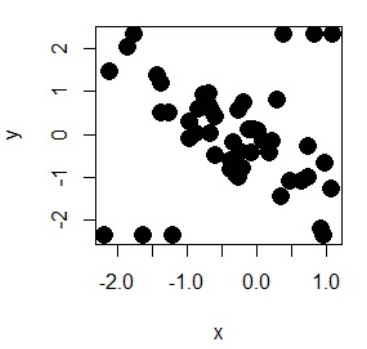
\includegraphics[width=0.5\linewidth]{ch-intro/figures/me2plot}
		\caption[A plot of data that exhibits a negative linear trend but fails the Pearson correlation test.]{A plot of data that exhibits a negative linear trend but fails the Pearson correlation test. The code for this analysis may be found in Appendix~\ref{sec:appendicies:me2plot}}
		\label{fig:intro:me2plot}
	\end{center}
\end{figure}

Notice that the analyst used a common test of linear correlation, and the data is clearly linear. The test, however, did not indicate that there was a significant relationship among the two variables; it was only after the data was plotted that this relationship was immediately noticed. Indeed, the data used in these examples was purposefully constructed to be dependent but bypass common tests for dependency. However, if it is possible to construct datasets in one-dimension that evade commonly-used numerical methods, it is believable that it is even easier to construct analogous datasets in higher dimensions.
